\documentclass[11pt,twocolumn]{article}
\usepackage{amssymb,amsmath}
\usepackage{dsfont}
\usepackage{times}
\usepackage[left=1in, right=1in, top=1in, bottom=0.5in, includefoot]{geometry}
\setlength\parindent{0.25in}
\setlength\parskip{1mm}

% This package is for including our graph
\usepackage{graphicx}

% This package is for the write-up for node code
\usepackage{pseudocode}

\title{Learning the Perfect Strategy for Tic-Tac-Toe with Gossip}
\author{Patrick Trinkle \& Mike Corbin\\
Dept. of Computer Science and Electrical Engineering,\\
University of Maryland Baltimore County,\\
Baltimore, MD, 21250\\
\texttt{\{tri1|corbin2\}@umbc.edu}}
\date{December 1st, 2009}

\begin{document}
\twocolumn[
  \begin{@twocolumnfalse}
    \maketitle
    \begin{abstract}
      Gossip is a robust protocol for nodes interacting in an unstructured network.  We apply this protocol to a set of nodes actively trying to solve a problem by interacting with each other.  The nodes are learning the perfect strategy for the game, Tic-Tac-Toe.  As the nodes play each other and try different strategies they move towards a perfect strategy, or one that does not lose.
    \end{abstract}
  \end{@twocolumnfalse}
  ]

\section{Motivation}

The gossip protocol dictates that nodes on the network select other nodes in the network to share information.  The information shared is typically small and the sharing is not necessarily bidirectional.  A node may have information it wishes to send off to other nodes in the network; a rumor.  As each node in the network learns the rumor it then finds other nodes to tell.  At each step in the rumor-spreading, the state of one or both of the nodes changes.  Within $O(\lg N)$ steps all nodes should know the rumor.  There are many variations in the system which can determine the effectiveness of the gossip system.  These variables include: what a node does if it pings a node that already knows the rumor; what a node does if it has been waiting around--should it ask if there is a rumor; whether the node choices are random from the network or from a neighbor list \cite{Birm2007}.

Erlang provides a stable distributed system and development environment.  Therefore it is a good choice for developing applications that utilize the gossip protocol.  However, it does have a limitation with the memory management system whereby all parameters to the recursive functions required are copied at each call{\bf \em{ Is this true?}}.  This downside makes Erlang a more suitable choice for rapid prototyping a system versus building a final program \cite{Erlang}.

\section{Background}

Gossip protocol systems do not strictly compute aggregate calculations, but can also disseminate information.  A system can manage data replicas as well as routing tables with gossip.  Nodes can use simple communication with other randomly selected nodes whereby one or both nodes change state after the information exchange.  These systems benefit from small communication requirements and do not require reliable communication.  Aggregate problems also converge in $O(\lg N)$ time to an estimate of the calculation.  These calculations can be anything that is composable, such as the average, variance, count.  Gossip can also estimate some problems that require complete knowledge (hollistic problems) \cite{Birm2007}.

\subsection{Erlang as a Distributed Environment}

Erlang was developed by Ericsson for robust, real-time concurrent systems.  Interprocess communication is abstracted away into a rather simple system to aid development.  Also, because Erlang is a functional language all code is written to run recursively {\bf {\em Is this true?}}.  Parameters are copied at each function call in the recursion which makes it unsuitable for developing systems which require larger data structures {\bf {\em Is this true?}}.  Erlang provides a simple platform for developing concurrent code.  Each process is spawned to run a function, similarly to fork()ing processes in a standard system or spawning threads.  A running system supports code modules being recompiled and injected without stopping the system, which aids in real-time upgrades and debugging \cite{Erlang}.

\section{Early Experiments}

Before determining which problem to address with the gossip protocol, we built several relatively small-scale applications in Erlang.  These applications allowed us to further understand the variables involved in a distributed system, such as one using the gossip protocol.  An initial application was built which simply shared a rumor.  To stop the rumor spreading the nodes would quit with certain probability upon contacting a node, which already knew the rumor.  From this code base, two applications where quickly developed.  They both built a spanning tree with gossip: in the first application the nodes tracked their parent; in the second the parents tracked their children.  Nodes discontinued the hunt for available children based on a certain probability after finding a node that was already in the tree.  Two variations of the average aggregate were also programmed.

These small programs provided useful feedback on the innerworkings of gossip as well as Erlang.  This feedback included how many nodes our systems could run and provide the illusion of concurrency, as well as how much each node could use for state before impacting performance and eventually crashing the Erlang system.

\subsection{Variables}

Developing a distributed system involves tweaking certain system parameters.  If nodes seek rumors during run-time this can change the time required for complete knowledge or solution convergence.  Simultaneously, this may not be required.  When a node interacts with another node that already knows the rumor the node can quit spreading the rumor or initiating interactions.  However, if too many nodes quit too quickly then the rumor can die out before all the nodes know.  Therefore, there is tweaking in whether or not a node should quit at this point; not just the binary notion but there can be a range using probability and random number generators.  If a node contacts another node that knows the rumor (assuming they're spreading rumors) it can roll a die to determine whether it should quit.  This variable has a very strong impact on the amount of messages sent as well as how many nodes end up ignorant of the rumor.  How many iterations of the gossiping the system completes may be unknown, therefore having the nodes self terminate can be useful.  In our experiments we modified how likely a node was to quit spreading the rumor, but did not have nodes seeking rumors.

\subsection{Epidemic Rumor Spreading}

This application spreads one rumor though the network starting at a node identified as "node1."  As nodes are informed of the rumor they change state from DontKnow to KnowAndTell.  Each node, whose state is KnowAndTell uniformly randomly chooses another node in the network after 10ms.  If this randomly chosen node knows the rumor, then the node who tried spreading the rumor will "roll a die" to determine whether or not to quit spreading the rumor.  Varying how likely you are to quit can impact how many nodes in the end of the rumor iterations are in the state DontKnow.  It also impacts how many messages are sent.  Therefore if the system has bandwidth constraints, this may influence how likely a node will quit.  Table \ref{tab:RumorProbability} displays the results of varying the probability that a node will quit spreading the rumor upon interacting with a node that already knows the rumor.

\begin{table}[h]
\caption{Epidemic Rumor Spreading: 100 Nodes}
\centering
\begin{tabular}{c | r r}
Probability & Total Messages & DontKnow\\
\hline
0.01	& 10233 & 0\\
0.05	& 1932 & 0\\
0.10 & 108 & 79\\
0.20 & 295 & 34\\
0.30 & 382 & 45\\
0.40 & 138 & 67\\
0.50 & 162 & 40\\
0.60 & 30 & 85\\
0.70 & 17 & 91\\
0.80 & 30 & 85\\
0.90 & 25 & 87\\
\hline
\end{tabular}
\label{tab:RumorProbability}
\end{table}

\subsection{Spanning Tree Building}

Similary starting with the root node, "node1."  Each node in state KnowAndTell contacts other nodes at random and if they are not in the tree they become children of that node.  To ensure that this process terminates, if a node contacts another node already in the tree then this node will stop trying to find new children with certain probability.  A first version of this program has each node only track their parent.  This approach has drawbacks.  A major drawback is that information cannot be easily passed down the tree; but it can be sent up the tree.  However, it is more capable of sending information up the tree.  If you want to give all nodes information, then the nodes have to periodically ping their parent.  A second version of this program has each node tracking all children.  This requires more storage space on the nodes and doesn't scale well to large networks.  A hybrid version wherein, both parents and children are tracked was not built.

Because the testing machine can only emulate concurrency to a point, if too many nodes are used in the experiments programs then the trees will be very tall and thin with each node only having one child.  This is due to the sequential execution of the concurrent processes.  Each process picks a node at random and then the next process has a chance to execute, but the previous process may not have another chance to run again for a while--because of the seemlingly round-robin approach.  As each of the processes starts up and executes it finds a child and then may not run again for quite a while.

Building spanning trees with gossip is fairly robust and runs quickly.  However, the experimental programs we wrote did not take location into account when choosing the random nodes.

\subsection{Calculating the Average}

Provided that a set of N nodes all have some value $\chi_i$.  To calculate the average of the values in the network, each node will randomly chose another node in the network and share the values and then average.  This process is repeated until all the nodes in the network have the same value; which should be the average.  It was more practical in our experiments to not seek equality, but rather some $\epsilon$ of each other.  If a node is in a state where it doesn't seek other nodes and hears from a node with a different value it starts finding other nodes.  Our first model just transmits their value to the other node--kind of like bullying it.  The second model does a pair-wise value transmission.  Both projects quit seeking new numbers based on a dice roll after they find a node that matches another.  With the first project eventually everyone stops, but one node will remain seeking out other nodes.  This final node has to have a built-in timeout mechanism.  This timeout is necessary because eventually no one will ping the remaining node.  With pair-wise proper communication this extra time out is unnecessary.

Running several iterations of the models with varying behavior towards stopping provided interesting results.  Upon completion from a number of messages sent by each node; the nodes all were within 1.0 of each other.  This range allowed for us to set the $\epsilon$ to 1.0.  Within a reasonable number of iterations the nodes all converged.  Proving the number of steps for this was unimportant for our final and target project; Learning the Perfect Tic-Tac-Toe Strategy.

\section{Learning the Perfect Tic-Tac-Toe Strategy}

The goal of our Tic-Tac-Toe gossip algorithm is to simulate a population of people learning how to play Tic-Tac-Toe.  We start with a population of people with no tic-tac-toe strategy and one person that wants to play.  A person only knows the rules for tic-tac-toe and how to contact the other players.  Each game starts with one person requesting a game by sending his strategy to another person.  The person that receives the strategy then plays a game of Tic-Tac-Toe with themselves as player 1 and the requesting person as player 2.  After the game is over the strategy and record of both players are updated and both players then look for someone else to play a game with.  Each player continues to request games until they stop losing, then they stop asking other people to play.

Each player represents their strategy as a series of snapshots of a board, along with the move for that snapshot.  When checking a board against their strategy all reflections and rotations are checked in order to minimize the number of snapshots needed to store.  After each game the strategies of the two players are modified in the following way.  If one of the players wins both players first remove the moves of the losing player from their strategy, then add the moves from the winning player into their strategy.  When there is a draw both players keep the moves from the second player, and no moves are removed.  The wins, losses, and draws are updated for each player after each game.  If the player loses: its wins, losses, and draws are reset to zero in order to make checking for the stoping strategy easier.

Given two nodes: $i$ \& $j$ in the set of nodes.  Node$i$ randomly choses a node$j$ to play Tic-Tac-Toe with.  $X$ is the set of moves, whereby $X[i]$ is the set of moves for node$i$.  The following algorithm describes this interaction:

\begin{pseudocode}[shadowbox]{Tic-Tac-Toe}{i,j}
\IF i \THEN
 \BEGIN
  \CALL{SendStrategy}{X[i], j}\\
  \CALL{ParseResponse}{X[i]}\\
  \IF win \THEN
   Wins \GETS Wins + 1
  \ELSEIF draw \THEN
   Draws \GETS Draws + 1
  \ELSE
   \BEGIN
    Losses \GETS 0\\
    Draws \GETS 0\\
    Wins \GETS 0\\
   \END
 \END
\ELSEIF j \THEN
 \BEGIN
  M \GETS \CALL{PlayGame}{X[i], X[j]}\\
  \IF i \space \mbox{wins} \THEN
   \BEGIN
    X[i] \GETS X[i] - M_{loss}\\
    X[j] \GETS X[j] - M_{loss}\\
    X[j] \GETS X[j] + M_{win}\\
   \END
  \ELSE \THEN
   \BEGIN
    X[j] \GETS X[j] - M_{loss}\\
    X[i] \GETS X[i] - M_{loss}\\
    X[i] \GETS X[i] + M_{win}\\
   \END \\
  \IF win \THEN
   Wins \GETS Wins + 1
  \ELSEIF draw \THEN
   Draws \GETS Draws + 1
  \ELSE
   \BEGIN
    Losses \GETS 0\\
    Draws \GETS 0\\
    Wins \GETS 0\\
   \END \\
  \CALL{SendResponse}{X[i], i}\\
 \END
\end{pseudocode}

Modifying the strategies in this way promotes population growth by keeping moves that lead to wins and draws for the second player, and removing moves that lead to losses.  It also keeps first player moves that lead to wins which provide more opportunities for people to find ways to stop them.  

There are two variables that modify the way this program runs.  The first is the number of nodes and the second is how many wins plus draws are needed before the process stop asking for additional games.  Both variables lead to more overall games the first by increasing the number of nodes playing, and the second by increasing the number of wins plus draws needed before stopping.

Figure \ref{fig:500nodes_windraw} displays the total wins and draws of a population of 500 nodes throughout a run of the algorithm.  The total number of wins and draws increase slowly over the first half of the graph while each process works on a strategy.  The slow increase is caused by the fact we reset the wins and draws to zero each time a process loses.  The wins and draw then increase faster once the process develop a strategy that is harder to beat.  When a perfect strategy is finally found the wins and draws increase exponentially as the process tests its strategy out to make sure it can't lose.

% Not sure why it won't place the image across both columns
\begin{figure*}[h]
\centering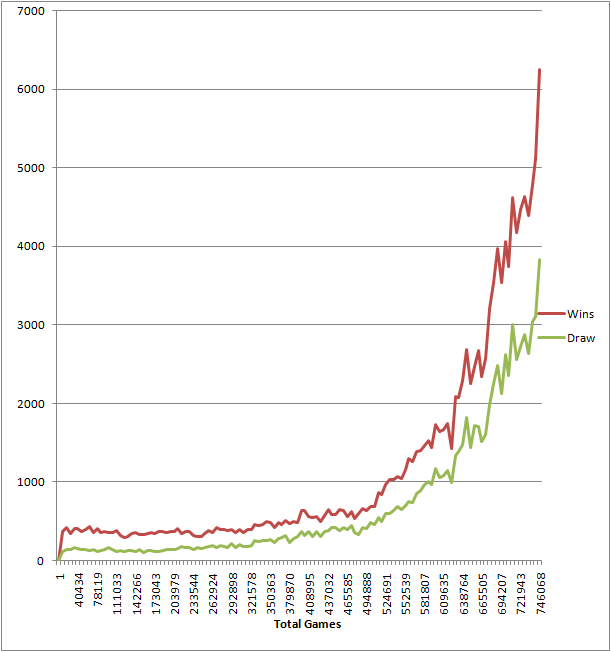
\includegraphics[keepaspectratio=true,scale=0.85]{500nodes_winsdrawpergames.png}

\caption{500 nodes}
\label{fig:500nodes_windraw}
\end{figure*}

\section{Future Work}

In this system the nodes work together with gossip to reach a shared goal.  This approach, wherein many nodes collectively and interactively work towards a shared goal can be applied to problems other than learning game strategies.  Further work can address how much interaction is required for certain systems to progress.  This approach can be applied to intelligent systems which process raw data to build analyzers.  The nodes can exchange these analyzers or processes with each other to build a better data processor.  A query can also be handled in a similar method whereby the nodes pass the query around as the rumor and contribute what they know of a response.

If the nodes are parsing large sets of text and building semantics and contexts for the contents, they can pass these around with the other nodes.  This improves the overall state of the parsers, as well as allows the work of building semantics to be distributed and shared among the nodes.

Systems can build up their own sketches or estimates of their status or data and then gossip this information in a similar fashion to the learning problem.  This would directly apply if the status of the node changed as the node's understanding of the data improved.

Building a Minimum Spanning Tree variation using gossip would require cost data  be included as well as knowledge of the node's parent.  The node would randomly interrogate other nodes on the network to determine if they would be a lower cost parent.  Provided there was a mechanism to avoid generating cycles; this implementation would be an interesting experiment using gossip.

\begin{thebibliography}{10}
\bibitem[Birm2007]{Birm2007}K. Birman, ``The promise, and limitations, of gossip protocols," \emph{ACM SIGOPS Oper. Syst. Rev.}, pp 8-13, 2007
\bibitem[Erlang]{Erlang}http://www.erlang.org/
\end{thebibliography}

\end{document}
